\documentclass[aspectratio=169,10pt]{beamer}

\usepackage{amsmath,amssymb}
\usepackage{graphicx}
\usepackage{caption}
\usepackage{braket}
\usepackage{biblatex}
\addbibresource{ref.bib}
\setbeamerfont{footnote}{size=\tiny}
\usetheme{CambridgeUS}
\usecolortheme{seahorse}
\usefonttheme{serif}
\pgfdeclareimage[height=0.5cm]{university-logo}{logo.png}
\logo{\pgfuseimage{university-logo}}

\title{Quantum Error Correction}
\subtitle{Experiments Realization}
\author{ZhangAiqiang}
\institute{Tsinghua University}
\date{\today}
\begin{document}
\begin{frame}
    \titlepage
\end{frame}
\begin{frame}
    \frametitle{Content}
    \tableofcontents
\end{frame}
\section{Theory}
\begin{frame}
    \frametitle{QEC Theory}
    \begin{columns}
        \begin{column}{0.5\textwidth}
            \begin{figure}
                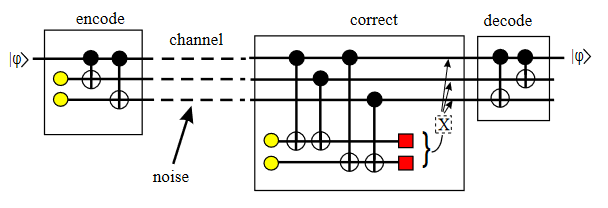
\includegraphics[width=\columnwidth]{figure/3bit.png}
                \caption{3 bit code QEC example}
            \end{figure}
            \begin{block}{Steps of QEC}
                \begin{enumerate}
                    \item encode $\psi$ to 3 bits
                    \item detect sydrome and error
                    \item error correction and decode
                \end{enumerate}
            \end{block}
        \end{column}
        \begin{column}{0.5\textwidth}
        \begin{figure}
            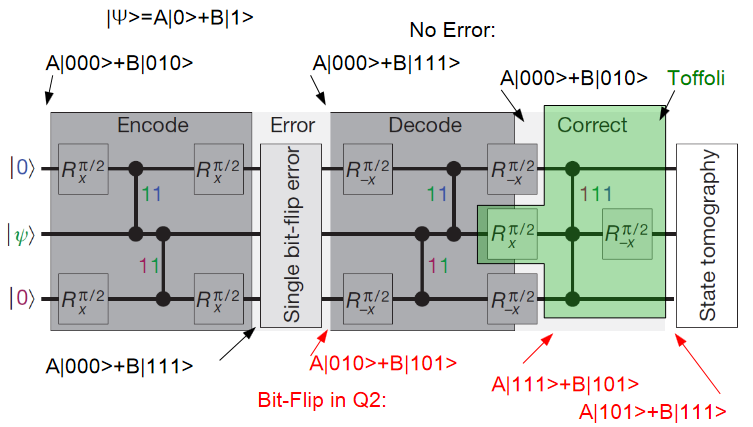
\includegraphics[width=0.9\columnwidth]{figure/toffoli.png}
            \caption{toffoli gate in QEC example}
        \end{figure}
        \begin{block}{Toffoli Gate}
            Toffoli Gate substitute the error detect and error correction.    
        \end{block}
        \end{column}
    \end{columns}
\tiny{Steane. A Tutorial on Quantum Error Correction}
\tiny{Superconducting circuits: Toffoli gate and error correction}
\end{frame}
\begin{frame}
    \frametitle{Surface Code}
    \begin{columns}
        \begin{column}{0.38\textwidth}
            \begin{figure}
                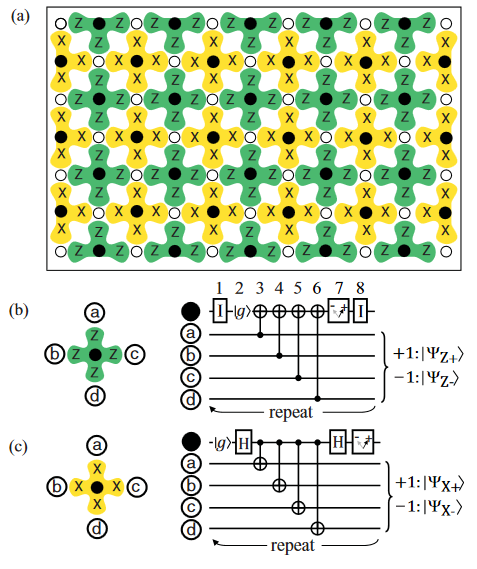
\includegraphics[width=\columnwidth]{figure/surfacecode.png}
                \caption{Surface code}
            \end{figure}
        \end{column}
        \begin{column}{0.6\textwidth}
            \begin{block}{Surface Code}
            \begin{enumerate}
                \item data qubit: open circle
                \item measurement-Z qubit: green solid circle
                \item measurement-X qubit: orange solid circle
            \end{enumerate}

            relative tolerance to local errors.
        \end{block}
        \end{column}
    \end{columns}
\tiny{Fowler. Surface codes: Towards practical large-scale quantum computation}
\end{frame}
\section{Experiments}
\subsection{3 bit code}
\begin{frame}
    \frametitle{Trapped Ions}
    \begin{columns}
        \begin{column}{0.45\textwidth}
            \centering
            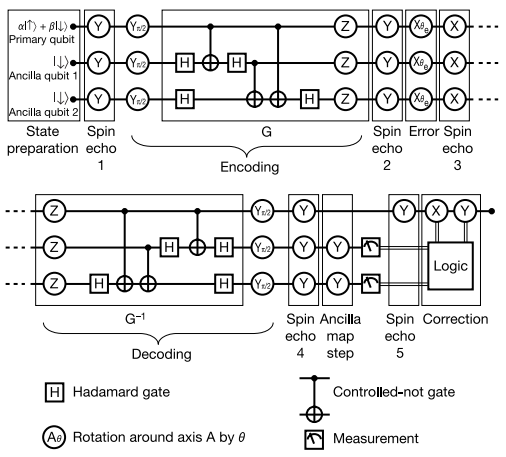
\includegraphics[width=\columnwidth]{figure/qec.png}
        \end{column}
        \begin{column}{0.55\textwidth}
            \centering
            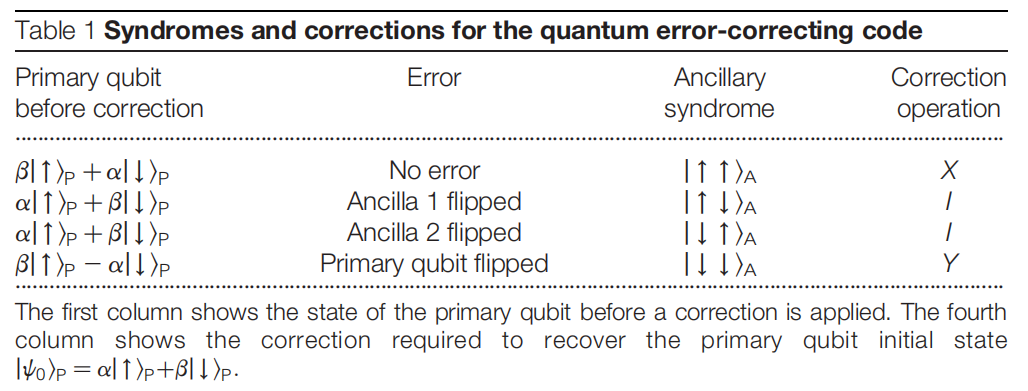
\includegraphics[width=\columnwidth]{figure/qec11.png}
            \begin{itemize}
                \item Measurement: resonnance fluorescence, $\ket{\downarrow}$ fluoresces whereas $\ket{\uparrow}$ not
                \item Use sydrome of ancilla to correct the error.
            \end{itemize}
        \end{column}
    \end{columns}
\tiny{Chiaverini. Realization of quantum error correction.}
\end{frame}
\begin{frame}
    \frametitle{Trapped Ions}
    \begin{columns}
        \begin{column}{0.55\textwidth}
            \centering
            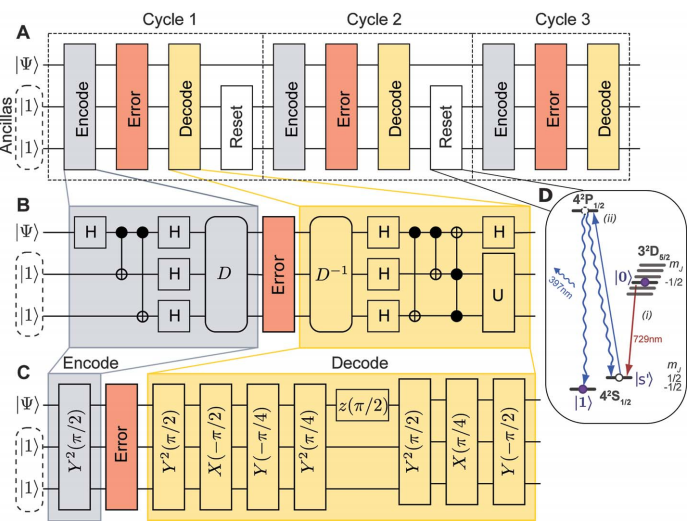
\includegraphics[width=\columnwidth]{figure/qec2.png}
        \end{column}
        \begin{column}{0.45\textwidth}
            \begin{enumerate}
                \item Initialization: optical-pumping technique.
                \item Toffoli Gate.
                \item Three consecutive correction cycles.
            \end{enumerate}
        \end{column}
    \end{columns}
\tiny{Schindler.Experimental Repetitive Quantum Error Correction}
\end{frame}
\begin{frame}
    \frametitle{Superconduct Qubit}
    \begin{columns}
        \begin{column}{0.45\textwidth}
            \centering
            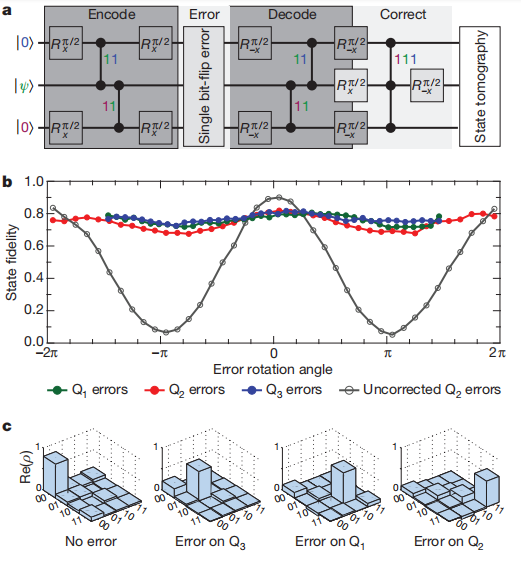
\includegraphics[width=\columnwidth]{figure/qec3.png}
        \end{column}
        \begin{column}{0.55\textwidth}
            \centering
            \begin{block}{}
                \begin{enumerate}
                    \item c: Two-qubit density matrices($\rho$) of the ancillas after each of the four possible full bit-flip errors has occurred.
                \end{enumerate}
            \end{block}  
        \end{column}
    \end{columns}
\tiny{Reed. Realization of three-qubit quantum error correction with superconducting circuits}
\end{frame}
\subsection{Surface Code}
\begin{frame}
    \frametitle{Surface Code}
    \begin{columns}
        \begin{column}{0.5\textwidth}
            \centering
            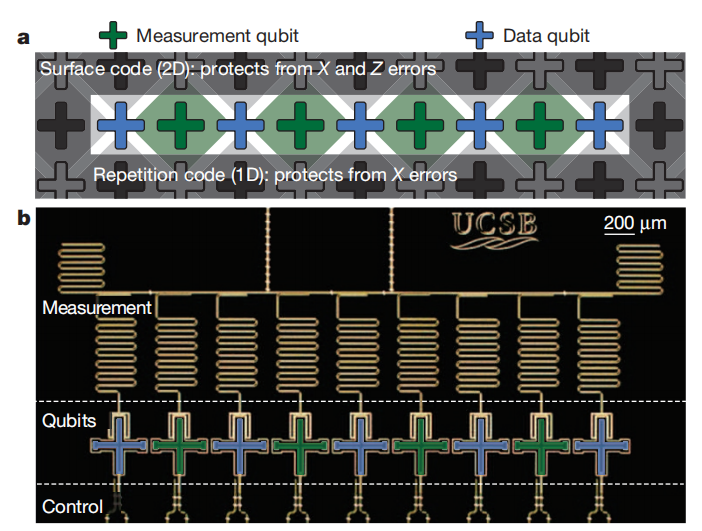
\includegraphics[width=\columnwidth]{figure/surface.png}
        \end{column}
        \begin{column}{0.5\textwidth}
            \centering
            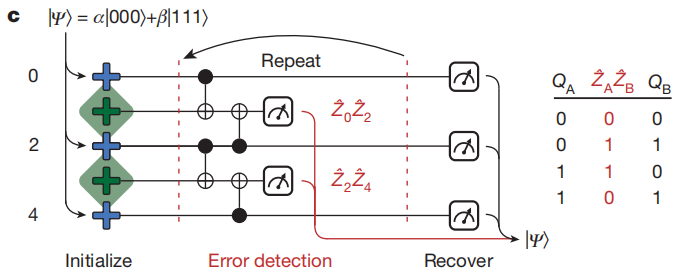
\includegraphics[width=\columnwidth]{figure/surface1.png}
            \begin{enumerate}
                \item 1D variant of the surface code, 9 qubits.
                \item The repetition code algorithm detect bit-flips.
            \end{enumerate}
        \end{column}
    \end{columns}
\tiny{Kelly. State preservation by repetitive error detection in a superconducting quantum circuit}
\end{frame}
\begin{frame}
    \frametitle{Surface Code}
    \begin{columns}
        \begin{column}{0.5\textwidth}
            \centering
            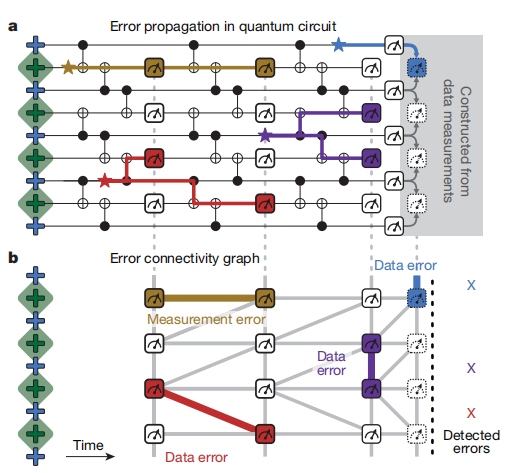
\includegraphics[width=\columnwidth]{figure/surface3.png}
        \end{column}
        \begin{column}{0.5\textwidth}
            \centering
            \begin{block}{Error propagation and identification}
                \begin{description}
                    \item examples of errors 
                    \item connectivity graph for the quantum circuit
                \end{description}
            \end{block}
            Fedelity: 
        \end{column}
    \end{columns}
\tiny{Kelly. State preservation by repetitive error detection in a superconducting quantum circuit}
\end{frame}


\section{Discuss}
\begin{frame}
    \frametitle{Discuss}
    \begin{enumerate}
        \item QEC has been realized physically in trapped ion and superconduct qubit.
        \item 
    \end{enumerate}
\end{frame}

\begin{frame}
    \centering{THANKS!}
\end{frame}
\end{document}